\documentclass{../../meta/tudscript}
\begin{document}
    \setcounter{section}{14}
    \setcounter{subsection}{1}

    \ilmath{Ord (M) &:= \Set{S \subseteq M \times M \mid S \text{ Ordnungsrelationen auf } M}\\
    LO (M) &:= \Set{S \in Ord (M) \mid S \text{linear}}}

    Ein Element $x \in M$ heißt:\\
    \ilmath{\text{\underline{maximal} in (M, R) } :\iff \forall y \in M: xRy \implies x = y}

    \ilmath{\text{\underline{minimal} in (M, R) } :\iff \forall y \in M: yRx \implies x = y}

    
    \ssect{Lemma}
        Sei (M, R) geordnete Menge. $a, b \in M$ unvergleichbar in $(M,R)$.
        Dann ist
        \ilmath{R_{a, b} := R \cup \Set{(x, y) \in M \times M: aRx \land bRy}}
        eine \underline{Ordnungserweiterung} von R mit $(a, b) \in R_{a, b}$

        \paragraph{Beweis}
	        Klar: $(a, b \in R_{a, b})$ und $R \subseteq R_{A, b}$
	        Insbesondere ist $R_{a, b}$ reflexiv.
        
	        \subparagraph{Transitivität}:
		            
		        Seien $x, y, z \in M$ mit $(x, y) \in R_{a, b}, (y, z) \in R_{a, b}$ 
		        
		        Fallunterscheidung:
		
		        \begin{enumerate}
		            \item $(x,y), (y, z) \in R \overset{R trans}{\implies} (x,z) \in R \overset{R \subseteq R_{a,b}}{\implies} (x, z) \in R_{a, b}$
		            \item $(x, y), (y, a), (b, z) \in R \overset{R trans}{\implies} (x, a), (b, z) \in R \implies (x, z) \in R_{a, b}$
		            \item $(x, a), (b, y), (y, z) \in R \overset{R trans}{\implies} (x,a), (b, z) \in R \implies (x,z) \in r_{a,b}$
		            \item $(x, a), (b,g),(y,a),(b,z) \in R \overset{R trans}{\implies} (b,a) \in R \lightning$ (Fall tritt nicht auf)
		        \end{enumerate}
		        
			Also $(x,z) \in R_{a, b}$.
		        
	        \subparagraph{Antisymmetrie}
		
		        Seien $x,y \in M$ mit $(x,y), (y,x) \in R_{a,b}$
		
		        Fallunterscheidung:
		
		        \begin{enumerate}
		            \item $(x,y), (y,x) \in R \overset{R antisym.}{\implies} x = y$
		            \item $(x,y), (y, a), (b,x) \in R \overset{R trans}{\implies} (b, a) \in R \lightning$
		            \item $(x,a), (b,y), (y,x) \in R \overset{R trans}{\implies} (b,a) \in R \lightning$
		            \item $(x,a), (b,y), (y,a), (b,x) \in R \overset{R trans}{\implies} (b,a) \in R \lightning$
		        \end{enumerate}
		        
		        Also $x = y$. Somit $R_{a, b} \in Ord (M) \hfill\square$
        
    \ssect{Lemma von Szpilrajn}
        Sei $(M, R)$ geordnete Menge und $(x,y) \in (M \times M) \setminus R$.
        Dann existiert eine lineare Ordnungserweiterung L von R mit $(x,y) \notin L$
		
        \paragraph{Beweis}
            
	        (Hier nur für M endlich.) Betrachte
	        \ilmath{\mathscr{A} := \Set{S \in Ord (M) \mid R \subseteq S \not\owns (x,y)}}
	        Dann $(\mathscr{A}, \subseteq)$ endliche geordnete Menege besitzt daher ein maximaels
	        Element $L \in \mathscr{A}$
	        
	        Annahme: L nicht linear.
	        
	        Dann gibt es $a, b \in M$ unvergleichbar in (M, L).
	        
	        Nach Lemma 14.2 \ref{14.2}: $K_{a,b}$ und $L_{b,a}$ Ordnungserweiterungen von $L \supseteq R$.
	
	        Wegen Maximalität von L:
	        \ilmath{L_{a,b} \notin \mathscr{A} \text{ d.h. } (x,y) \in L_{a,b} \cap l_{b,a}}
	
	        Da $(x,y) \notin L$, folgt $xLa, aLy$, somit $xLy$. Widerspruch! $\hfill\boxed{\lightning}$

       
    \ssect{Folgerung (Satz von Dushnik \& Miller)}
        Sei $(M,R)$ nichtleere geordnete Menge, Dann
        \ilmath{\exists \mathscr{L} \subseteq LO (M), \mathscr{L} \neq \emptyset, R = \bigcap \mathscr{L}}

    \ssect{Definition: Ordnungsdimension}
        Ist $(M, R)$ nicht-leer, endliche, geornete Menge, dann heißt
        \ilmath{dim ((M, R)) := dim (R) := min \Set{\mid \mathscr{L} \mid | \emptyset \neq \mathscr{L} \subseteq LO (M): R = \bigcap \mathscr{L}}}
        \underline{Ordnungsdimension} von (M,R) bzw. R.\\

        Sind $(M_0, \leq_0)$ und $(M_1, \leq_1)$ geordnete Mengen, dann heißt\\
        $\varphi: M_0 \rightarrow M_1$
        \ilmath{\text{ \underline{Ordnungserhaltent}} :\iff \forall x,y \in M_0: x \leq_0 y \implies \varphi (x) \leq_1 \varphi (y) &&}
        \ilmath{\text{ \underline{Ordnungsreflektierend}} :\iff \forall x,y \in M_0: \varphi (x) \leq_1 \varphi (y) \implies x \leq_0 y &&}
        
        Hier als Bsp.: Ordnungsbewahrend aber nicht Ordnungsreflektierend.\\
        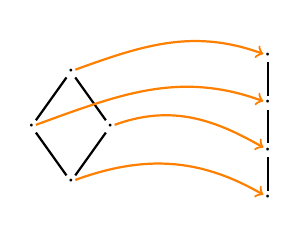
\begin{tikzpicture}
	        \node [inner sep=0pt] at (0, 0) (C0) {$\cdot$};
	        \node [inner sep=0pt] at (1, 0) (C2) {$\cdot$};
	        \node [inner sep=0pt] at (0.5, 0.7) (C1) {$\cdot$};
	        \node [inner sep=0pt] at (0.5, -0.7) (C3) {$\cdot$};
	        \draw [black, thick] (C0) -- (C1);
	        \draw [black, thick] (C0) -- (C3);
	        \draw [black, thick] (C2) -- (C1);
	        \draw [black, thick] (C2) -- (C3);
	        \node [inner sep=0pt] at (3, 0.9) (L0) {$\cdot$};
	        \node [inner sep=0pt] at (3, 0.3) (L1) {$\cdot$};
	        \node [inner sep=0pt] at (3, -0.3) (L2) {$\cdot$};
	        \node [inner sep=0pt] at (3, -0.9) (L3) {$\cdot$};
	        \draw [black, thick] (L0) -- (L1);
	        \draw [black, thick] (L1) -- (L2);
	        \draw [black, thick] (L2) -- (L3);
	        \draw [orange, thick, ->] (C1) to[out=20,in=160] (L0);
	        \draw [orange, thick, ->] (C0) to[out=20,in=160] (L1);
	        \draw [orange, thick, ->] (C2) to[out=20,in=150] (L2);
	        \draw [orange, thick, ->] (C3) to[out=20,in=150] (L3);
	        
        \end{tikzpicture}
        
        \ilmath{\text{ \underline{Ordnungseingebettet}} :\iff \varphi \text{ ordnungserhaltent und ordnungsreflektierend} &&}

        \ilmath{\text{ \underline{Isomorphismus}} :\iff \varphi \text{ surjektive Ordnungseinbettung} &&}\\

        Wir nennen $(M_0, \leq_0)$ isomorph zu $(M_1, \leq_1)$

        \ilmath{:\iff \exists \phi: (M_0, \leq_0) \rightarrow (M_1, \leq_1) \text{ Isomorphismus}}\\

        Das \underline{direkte Produkt} von geordneten Mengen $(L_1, \leq_1), \ldots, (L_n, \leq_n)$ ist die geordnete Menge

        \ilmath{\prod_{i = 1}^{n} (L_i, \leq_i) := (\prod_{i = 1}^n L_i, \leq)}
        mit $(x_1, \ldots, x_n) \leq (y_1, \ldots, y_n) :\iff \forall i \in \Set{1, \ldots, n}: x_i \leq_i y_i$\\
        für $(x_1, \ldots, x_n) (y_1, \ldots, y_n) \in \prod_{i = 1}^n L_i$.

    \ssect{Bemerkung}
        Ist $(M, \leq)$ nicht-leere, endliche, geordnete Menge, dann gilt:
        \ilmath{dim (M, \leq) := min \Set{n \in \bN \Large| \begin{aligned} &\; \exists (k_1, \leq_1), \ldots, (k_n, \leq_n) \text{ Ketten} \\ &\; \exists \varphi: (M, \leq) \rightarrow \prod_{i = 1}^n (L_i, \leq, i) \text{ Ordnungseinbettung} \end{aligned} } }
        %\ilmath{dim (M, \leq) := min \Set{n \in \bN \mid &\exists (k_1, \leq_1), \ldots, (k_n, \leq_n) \text{Ketten}:\\
        %		&\exists \varphi: (M, \leq) \rightarrow \prod_{i = 1}^n (L_i, \leq, i) \text{Ordnungseinbettung} } }

        \paragraph{Zum Beweis:}
            Siehe B. Ganter, Diskrete Mathematik: "Geordnete Mengen", Springer, 2013

    \ssect{Definition: Weite einer geordneten Menge} 
        Ist $(M; \leq)$ endliche, geordnete Menge, dann heißt:
        \ilmath{width (M, \leq) := max \Set{|A| \mid A \text{ Antikette in } (M, \leq)}}
        die \underline{Weite} von $(M, \leq)$.

   \ssect{Satz von Dilworth}
        Sei $(M, \leq)$ endliche, geordnete Menge. Dann:
        \ilmath{width (M, \leq) = min \Set{n \in \bN \mid \exists K_1, \ldots, K_n \text{ Ketten in } (M, \leq): M = \overset{n}{\underset{i = 1}{\cup}} K_i}}
\end{document}
